
%% bare_jrnl_compsoc.tex
%% V1.4a
%% 2014/09/17
%% by Michael Shell
%% See:
%% http://www.michaelshell.org/
%% for current contact information.
%%
%% This is a skeleton file demonstrating the use of IEEEtran.cls
%% (requires IEEEtran.cls version 1.8a or later) with an IEEE
%% Computer Society journal paper.
%%
%% Support sites:
%% http://www.michaelshell.org/tex/ieeetran/
%% http://www.ctan.org/tex-archive/macros/latex/contrib/IEEEtran/
%% and
%% http://www.ieee.org/

%%*************************************************************************
%% Legal Notice:
%% This code is offered as-is without any warranty either expressed or
%% implied; without even the implied warranty of MERCHANTABILITY or
%% FITNESS FOR A PARTICULAR PURPOSE! 
%% User assumes all risk.
%% In no event shall IEEE or any contributor to this code be liable for
%% any damages or losses, including, but not limited to, incidental,
%% consequential, or any other damages, resulting from the use or misuse
%% of any information contained here.
%%
%% All comments are the opinions of their respective authors and are not
%% necessarily endorsed by the IEEE.
%%
%% This work is distributed under the LaTeX Project Public License (LPPL)
%% ( http://www.latex-project.org/ ) version 1.3, and may be freely used,
%% distributed and modified. A copy of the LPPL, version 1.3, is included
%% in the base LaTeX documentation of all distributions of LaTeX released
%% 2003/12/01 or later.
%% Retain all contribution notices and credits.
%% ** Modified files should be clearly indicated as such, including  **
%% ** renaming them and changing author support contact information. **
%%
%% File list of work: IEEEtran.cls, IEEEtran_HOWTO.pdf, bare_adv.tex,
%%                    bare_conf.tex, bare_jrnl.tex, bare_conf_compsoc.tex,
%%                    bare_jrnl_compsoc.tex, bare_jrnl_transmag.tex
%%*************************************************************************


% *** Authors should verify (and, if needed, correct) their LaTeX system  ***
% *** with the testflow diagnostic prior to trusting their LaTeX platform ***
% *** with production work. IEEE's font choices and paper sizes can       ***
% *** trigger bugs that do not appear when using other class files.       ***                          ***
% The testflow support page is at:
% http://www.michaelshell.org/tex/testflow/


\documentclass[10pt,conference,onecolumn,compsoc]{IEEEtran}


\usepackage{hyperref}
\usepackage{enumitem}
\setlist[itemize]{leftmargin=3 cm}
\setlist[enumerate]{leftmargin=3cm}



% *** CITATION PACKAGES ***
%
\ifCLASSOPTIONcompsoc
  % IEEE Computer Society needs nocompress option
  % requires cite.sty v4.0 or later (November 2003)
  \usepackage[nocompress]{cite}
\else
  % normal IEEE
  \usepackage{cite}
\fi
% cite.sty was written by Donald Arseneau
% V1.6 and later of IEEEtran pre-defines the format of the cite.sty package
% \cite{} output to follow that of IEEE. Loading the cite package will
% result in citation numbers being automatically sorted and properly
% "compressed/ranged". e.g., [1], [9], [2], [7], [5], [6] without using
% cite.sty will become [1], [2], [5]--[7], [9] using cite.sty. cite.sty's
% \cite will automatically add leading space, if needed. Use cite.sty's
% noadjust option (cite.sty V3.8 and later) if you want to turn this off
% such as if a citation ever needs to be enclosed in parenthesis.
% cite.sty is already installed on most LaTeX systems. Be sure and use
% version 5.0 (2009-03-20) and later if using hyperref.sty.
% The latest version can be obtained at:
% http://www.ctan.org/tex-archive/macros/latex/contrib/cite/
% The documentation is contained in the cite.sty file itself.



% *** GRAPHICS RELATED PACKAGES ***
%
\ifCLASSINFOpdf
   \usepackage[pdftex]{graphicx}
 
\else
 
\fi
% graphicx was written by David Carlisle and Sebastian Rahtz. It is
% required if you want graphics, photos, etc. graphicx.sty is already
% installed on most LaTeX systems. The latest version and documentation
% can be obtained at: 
% http://www.ctan.org/tex-archive/macros/latex/required/graphics/
% Another good source of documentation is "Using Imported Graphics in
% LaTeX2e" by Keith Reckdahl which can be found at:
% http://www.ctan.org/tex-archive/info/epslatex/
%
% latex, and pdflatex in dvi mode, support graphics in encapsulated
% postscript (.eps) format. pdflatex in pdf mode supports graphics
% in .pdf, .jpeg, .png and .mps (metapost) formats. Users should ensure
% that all non-photo figures use a vector format (.eps, .pdf, .mps) and
% not a bitmapped formats (.jpeg, .png). IEEE frowns on bitmapped formats
% which can result in "jaggedy"/blurry rendering of lines and letters as
% well as large increases in file sizes.
%
% You can find documentation about the pdfTeX application at:
% http://www.tug.org/applications/pdftex









% *** PDF, URL AND HYPERLINK PACKAGES ***
%
\usepackage{url}
% url.sty was written by Donald Arseneau. It provides better support for
% handling and breaking URLs. url.sty is already installed on most LaTeX
% systems. The latest version and documentation can be obtained at:
% http://www.ctan.org/tex-archive/macros/latex/contrib/url/
% Basically, \url{my_url_here}.




\begin{document}

\title{Maze Database\\ for UTM CSCI 352}
%
%

% received ..."  text while in non-compsoc journals this is reversed. Sigh.

\author{Grace Looney\\Matthew Pugh% <-this % stops a space
}

\IEEEtitleabstractindextext{%
\begin{abstract}
The goal of our project is to create a maze game using WPF applications. We are planning for our game to be able to randomly cycle through at least five pregenerated mazes. Our target audience is gamers who enjoy solving puzzles and are looking for a short, fun diversion. 
\end{abstract}

}


% make the title area
\maketitle



\IEEEdisplaynontitleabstractindextext

\IEEEpeerreviewmaketitle



\section{Introduction}


For \textit{Maze}, we accomplished an interactive WPF application that involves computer generated mazes. We are using a Binary Algorithm to create the mazes due to its ability to create infinite sized mazes very quickly. The maze will be seen in an isometric view where the viewer will only be able to see a portion and the screen will move with the player. 

Maze is intended for people who enjoy puzzle games. It offers a simple distraction to the constant boredom most humans suffer from.  We hope our audience will achieve a sense of fulfillment out of our game because they solved a maze or multiple mazes. 

\subsection{Background}
We want to our maze to be 'perfect' and  'orthogonal' \cite{Pullen}. A 'perfect' maze means that the maze lacks loops and closed circuits. So the maze does not have any unreachable areas. In addition, 'perfect' implies that there is exactly one path. There are multiple ways to do this. For example, one of the easiest ways to achieve a perfect orthogonal algorithm is to a Binary Tree algorithm.  Although the Binary Tree algorithm is simple and fast, there is one con it is very biased due how it  creates the maze. Each cell carves the next cell by randomly choosing a cell that is either two directions which causes the product to have passages that lead diagonally from upper left to lower right. We overlooked this downside because of the ease of implementation.

We wanted to do this project because of the implementation of an algorithm that we learned in CSCI 325. In addition, this application allows us to gain an understanding of how game applications work.


\subsection{Challenges}
There were many challenges to this project. With the CONVID-19 outbreak, we lost the ease of the communication which was the first step of our mighty downfall. There were multiple challenges: implementing a way to view the maze, player movement, and the settings menu. The biggest challenge implementing a way to view the maze, because the algorithm only returns whether the cell is linked. Although we never accomplished the player movement. The Settings menu's challenges were diverse because we had to understand how to pass on the settings values that the user selected to other pages.

\section{Scope}
Our project is done when we have a 'perfect' 'orthogonal' maze application with a top-down view. In addition, the user will be able to view a menu with buttons that'll allow them to make binary tree maze and format it to be viewed top-down. 
\subsection{Stretch Goals:}
We completed 1 out 4 of our stretch goals.  The timer is half-way implemented. It shows a timer but when the user pauses the maze it does not stop the timer. We did not complete the \textit{scored} stretch goal, because of the timer issue and the inability to gather points. We minimally completed the \textit{music} stretch goal. The music does not continuously play, but it does restart every time the user opens a new window. The \textit{secret buttons} implementation was not attempted.
\begin{itemize}
\item Timed: The user can see how long it took them to complete that maze.
\item Scored: The user can earn points by collecting items across the maze.
\item Music: The user can have music while completing the maze.
\item Secret Buttons: The user can access special items or areas when standing on secret button

\end{itemize}


\subsection{Requirements}
For our requirements, we met a portion of them. We were able to complete all of the nonfunctional requirements. The application uses the binary tree algorithm to create a maze within one second on worst case scenario \ref{item:NF2}. For the \textit{scalability} \ref{item:NF1}, there is a global maze variable that a power user can adjust when they want a bigger or smaller maze. The functional requirements that we met are \ref{itm:F1},\ref{itm:F2},\ref{itm:F3}, and\ref{itm:F4}. The functional requirements that we did not meet: \ref{itm:F5}, \ref{itm:F6}, and \ref{itm:F7}. 
\subsubsection{Functional}
\begin{enumerate}
\item User needs to be able to view the GUI\label{itm:F1} 
\item User needs to be able to interact with the GUI\label{itm:F2} 
\item User needs to view the maze\label{itm:F3} 
\item User needs to be able to interact with the maze\label{itm:F4} 
\item Application needs to be able to save 3 games\label{itm:F5} 
\item Application needs to be able to load any of the three saved games \label{itm:F6}
\item Application will record high scores \label{itm:F7}
\end{enumerate}

\subsubsection{Non-Functional}
\begin{itemize}
\item Performance- Application will create mazes in a short amount of time\label{item:NF2} 
\item Scalability - Application will create mazes of different sizes\label{item:NF1}
\end{itemize}

\subsection{Use Cases}


We have seven use cases. \ref{UC:StartNewGame} is medium complexity because all this case required was transferring of the data values: size, settings choices. In addition, it needed to show a game screen after the \textit{New Game} button was clicked. \ref{UC:Customize} is medium complexity and $2_{nd}$ priority because it only requires an small understanding of how GUI works and how to transfer values from one page to the next. In addition, Customize does not impede any other use case, so this is why it has a low priority. \ref{UC:Save} is medium complexity and low priority because it's implementation only effects \ref{UC:Load} because Load calls upon the data that \ref{UC:Save} saved. \ref{UC:Scores} is low priority and medium difficulty because it does not affect any other use case. \ref{UC:Play} is high priority and very complex. Playing the game is the sole purpose of this project so its complexity and priority demonstrate this. \ref{UC:Credits} is listed as an easy task and low priority because it does not impede any other use case and its just an information window. 

\begin{table}
\centering
\begin{tabular}{|c|c|c|c|c|}
\hline
Use Case ID & Use Case Name & Primary Actor & Complexity & Priority \\
\hline \hline
1\label{UC:StartNewGame} & Start New Game & Gamer & Med & 1\\
2\label{UC:Customize} & Customize Maze & Gamer & Med & 2\\
3\label{UC:Save} & Save Game & Gamer & Med & 3\\
4\label{UC:Load} & Load Game & Gamer & Med  &3\\
5\label{UC:Scores}  & Calculate High Scores & Computer & Med & 3\\
6\label{UC:Play}  & Play Game & Gamer & Hard & 1\\
7\label{UC:Credits} & View Credits & Gamer & Easy & 4\\
\hline

\end{tabular}
\caption{Use case table}
\label{tab:useCaseIndex}
\end{table}


\begin{itemize}
\item[Use Case Number:] 1\ref{UC:StartNewGame}
\item[Use Case Name:] Start New Game 
\item[Description:] The gamer on our WPF application wants to play a new game. They will click the "New Game" Button, and this will start the off the Binary Tree algorithm to create a new maze. In addition, the maze will display after algorithm is completed. 
\item[Pre-conditions:]
\begin{itemize} 
\item Maze is downloaded
\item Maze has been opened
\end{itemize}

\item[Post-conditions:]
\begin{itemize} 
\item New game will be started
\end{itemize}
\item[Invariants:]
\begin{itemize} 
\item New game function is working properly
\item Game runs as it is meant to
\end{itemize}

\item[Process:]
\begin{enumerate}
\item Select New Game from the main menu
\item Play game
\end{enumerate}

\begin{itemize}
\item[Use Case Number:] 2
\item[Use Case Name:] Customize Maze
\item[Description:] The gamer on our WPF application wants to edit their maze appearance or the sounds of the maze. The gamer clicks the "Settings" button. This will take the gamer to the settings menu, so they can customize the maze appearance.

\item[Pre-conditions:]
\begin{itemize} 
\item Maze is downloaded
\item Maze has been opened
\end{itemize}

\item[Post-conditions:]
\begin{itemize} 
\item Current maze theme will be updated
\end{itemize}
\item[Invariants:]
\begin{itemize} 
\item Theme function is working properly
\item Music function is working properly
\item Customize function is working properly

\end{itemize}
\end{itemize}

\item[Process:]
\begin{enumerate}
\item Select settings from home screen
\item If desired theme already exists, then select it from the Theme menu
\item If desired theme does not exist, then move to the Customize menu
\item Select desired color for maze walls
\item Select desired color for maze floor
\item Select desired music setting from the Music menu
\item Save maze settings
\end{enumerate}
\begin{itemize}
\item[Use Case Number:] 3
\item[Use Case Name:] Save Game
\item[Description:] The gamer on our WPF application wants to save their unfinished maze. The gamer selects in the "save" button from the game view. They will be able to select one of the save spaces to save their maze to that memory spot.
\item[Pre-conditions:]
\begin{itemize} 
\item Maze is downloaded
\item Maze has been opened
\end{itemize}

\item[Post-conditions:]
\begin{itemize} 
\item Current game is saved in desired save slot
\end{itemize}
\item[Invariants:]
\begin{itemize} 
\item Pause function is working properly
\item Save function is working properly
\end{itemize}

\item [Process]
\end{itemize}
\begin{enumerate}
\item Click pause button
\item Click save button
\item Select a save slot
\item If save slot is currently being used, then decide whether or not to overwrite the previous save
\item Return to pause menu
\item End current game

\end{enumerate}

\end{itemize}
\subsection{Interface Mockups}
\begin{center}
\begin{figure}[ht!]
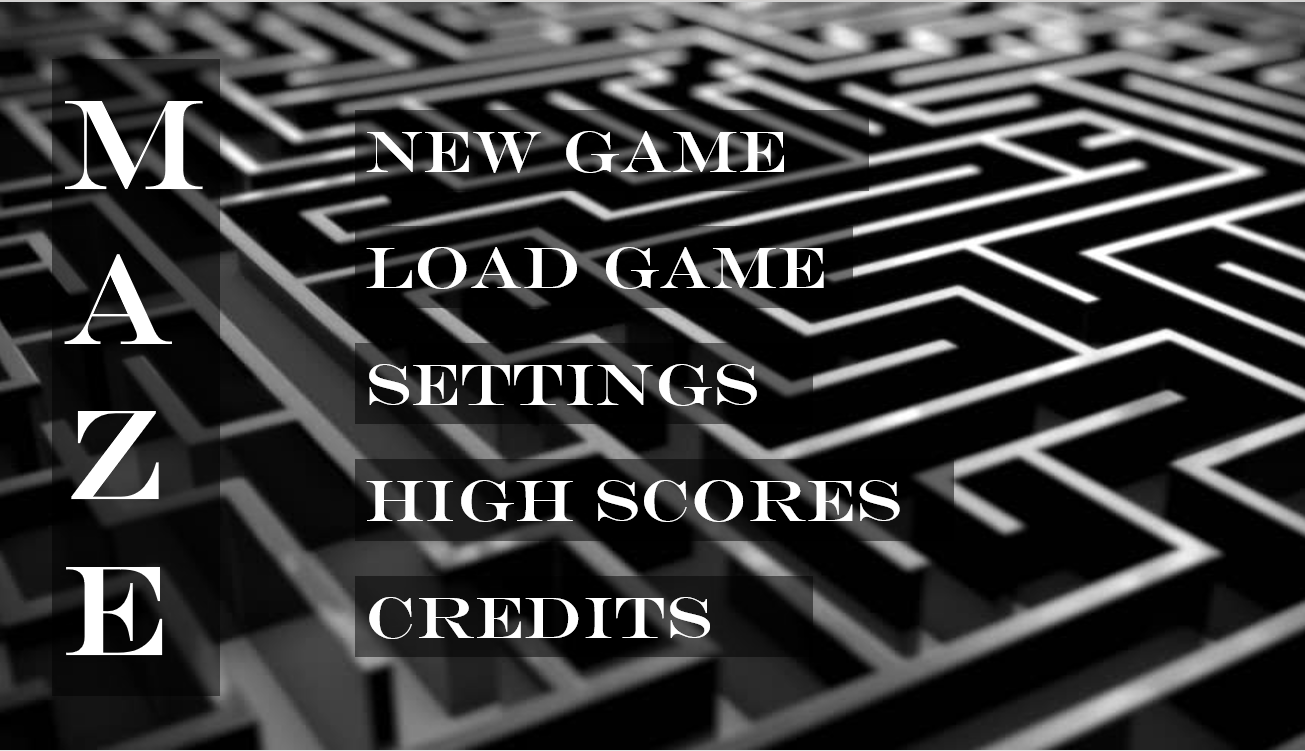
\includegraphics[height=150px, width=250px]{interface/Interface-Menu.png}
\caption{This is the Menu, There are five buttons on this menu. All of them lead to another window. Users will see this screen first. The first button, \textit{New Game}, transports the user to \ref{Start of Maze}. The second button, \textit{Load Game}, transports the user to \ref{Load}.The second button, \textit{High Scores}, transports the user to \ref{High Scores}. The \textit{Credits} button transports the user to \ref{Credits}. The \textit{Settings} button transports the user to \ref{Settings}.}
\label{Menu}
\end{figure}

\begin{figure}[ht!]
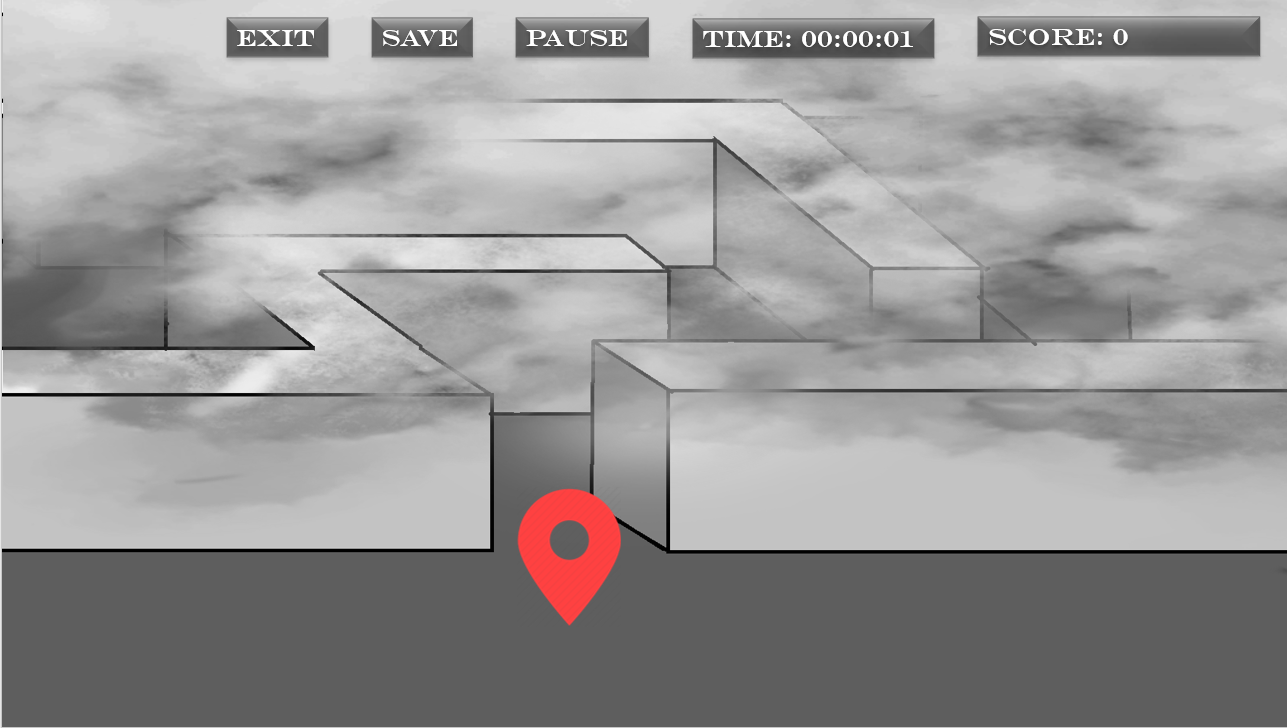
\includegraphics[height=150px, width=250px]{interface/Interface-BeginMaze.png}
\caption{This is the screen where the "New Button" \ref{Menu} transports the user to. In this form, There are three buttons: \textit{Reset}, \textit{Save Image} and \textit{Draw Path}. \textit{Reset} button resets the current maze to the original view. \textit{Save image} button saves an image to the users specified location. \textit{Draw Path} shows the route to take to finish the maze.}
\label{Start of Maze}
\end{figure}
\begin{figure}[ht!]
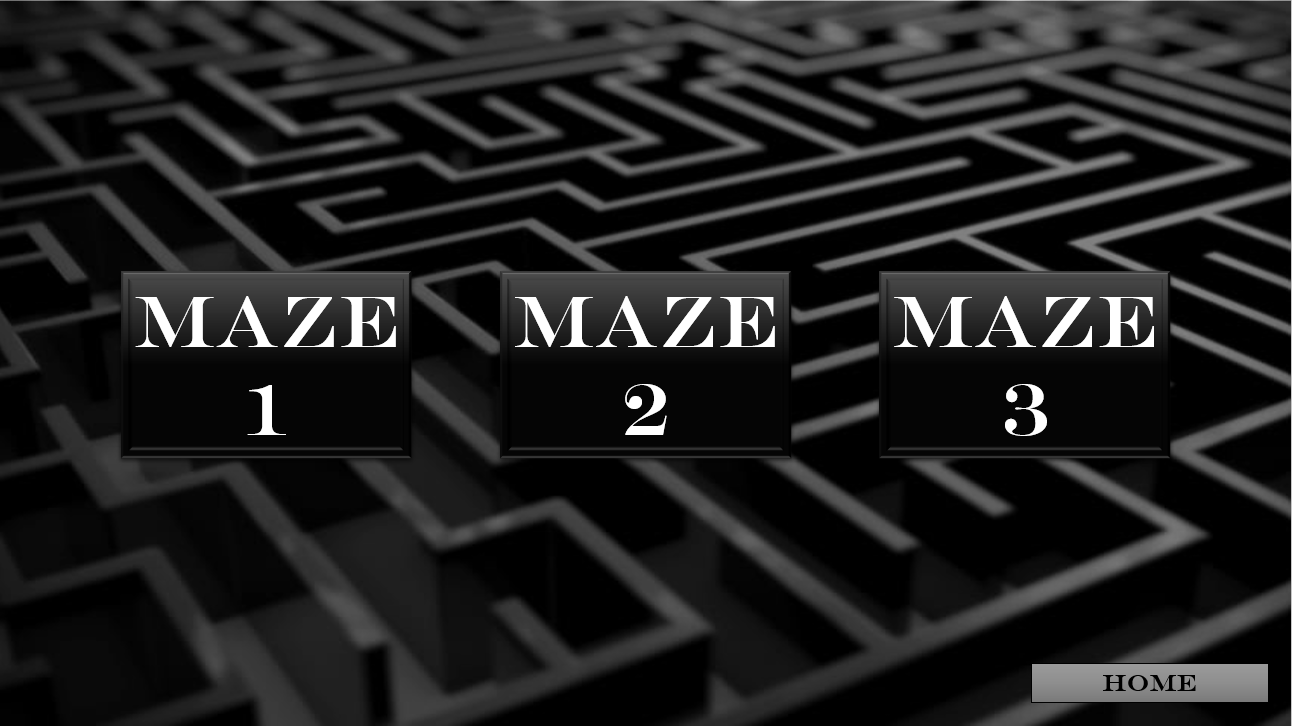
\includegraphics[height=150px, width=250px]{interface/Interface-Load.png}
\caption{This is the Load Screen that will appear after they select the button \textit{Load Game}. There are three buttons on this screen, each will load a save game.}
\label{Load}
\end{figure}
\begin{figure}[ht!]
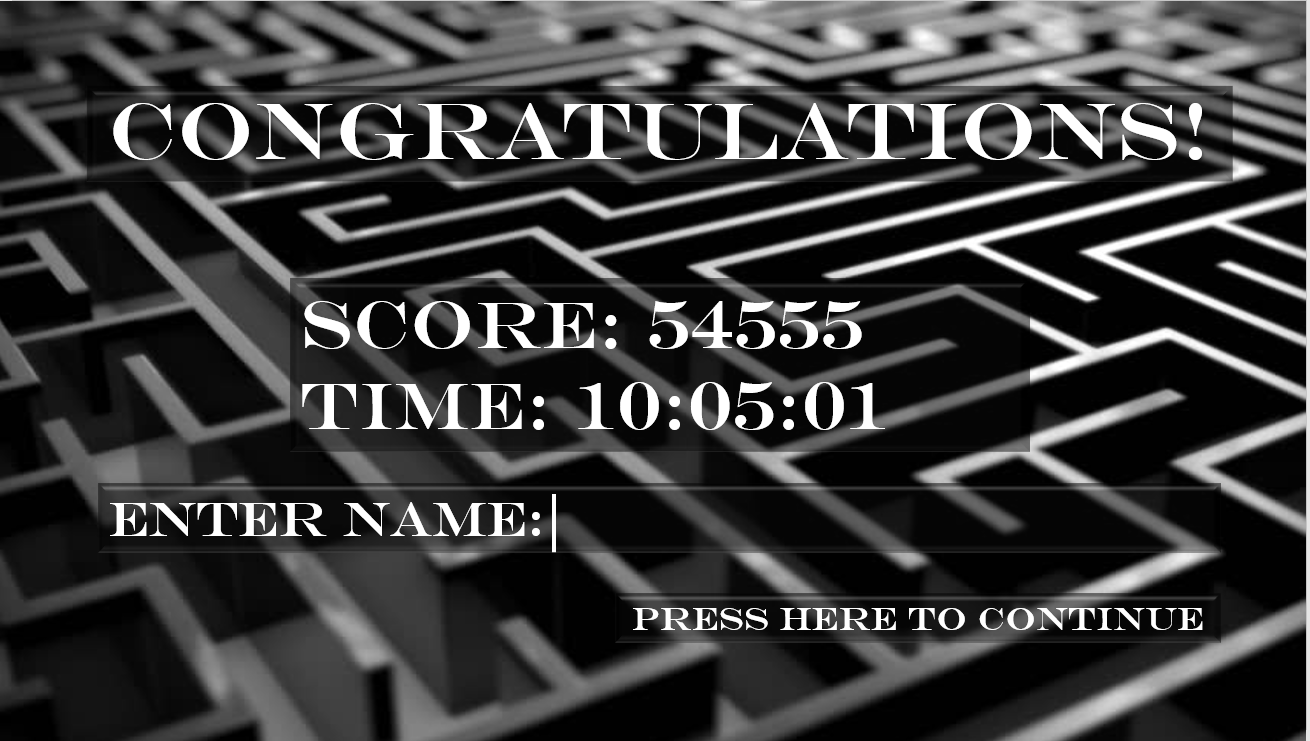
\includegraphics[height=150px, width=250px]{interface/Interface-Finish.png}
\caption{This is the screen that will be shown after the Maze game has finished}
\label{Finish Screen}
\end{figure}
\begin{figure}[ht!]
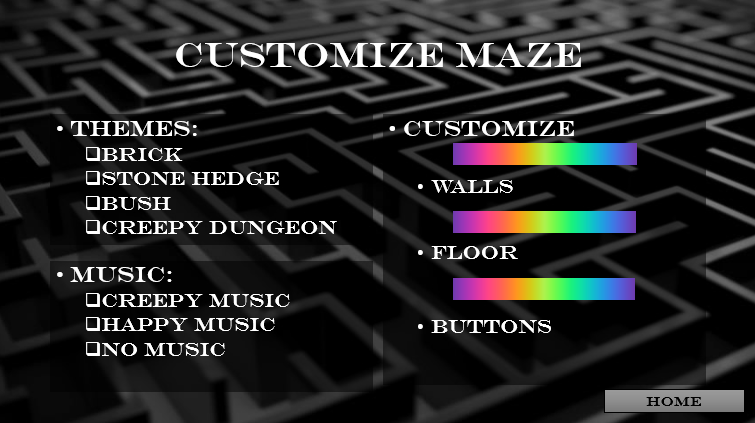
\includegraphics[height=150px, width=250px]{interface/Interface-Customize.png}
\caption{This is the Customize Menu}
\label{Settings}
\end{figure}
\begin{figure}[ht!]
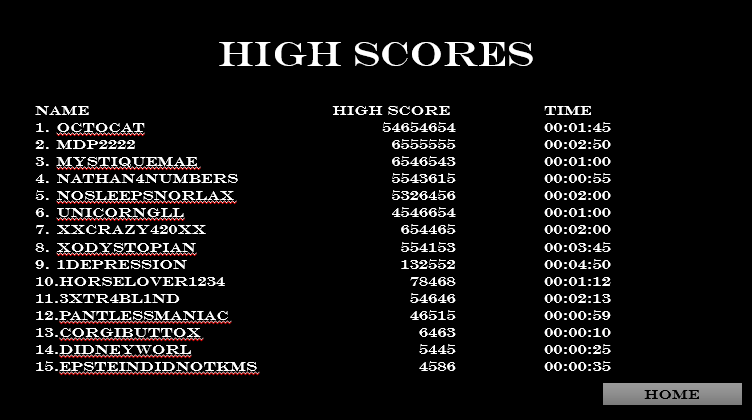
\includegraphics[height=150px, width=250px]{interface/Interface-HighScores.png}
\caption{This is the High Score Screen. It shows the current fake high scores.}
\label{High Scores}
\end{figure}
\begin{figure}[ht!]
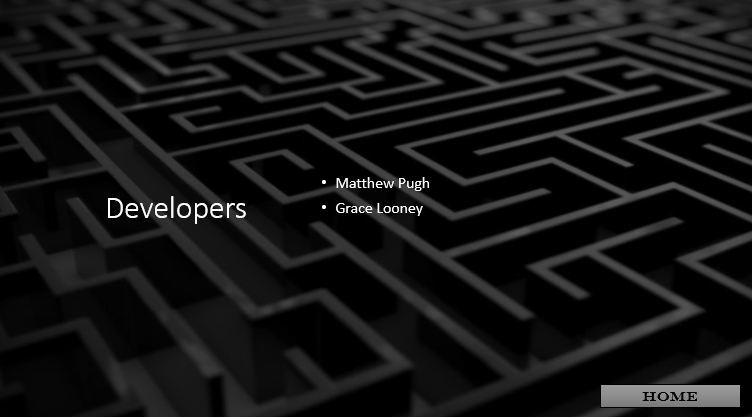
\includegraphics[height=150px, width=250px]{interface/Interface-Credits.png}
\caption{This is the Credits screen. It shows who is responsible for this catastrophe.}
\label{Credits}
\end{figure}
\end{center}
\clearpage
\section{Project Timeline}

Maze Game Timeline: (refer to Table 2 for a more detailed schedule)
\begin{enumerate}
\item Requirements: January 20 - February 27
\item Design: February 28 – March 31
\item Implementation: April 1 – April 20
\item Verification: April 21 – April 26
\item Maintenance: April 26 - onward
\end{enumerate}
Explanation: 
\begin{itemize} 
\item Requirements
\begin{itemize}
\item Teams formed. Began planning what we wanted the game to do and look like. Decided what features we need/want to implement.
\end{itemize}
\item Design
\begin{itemize}
\item Planned out the programming structure of the maze game. Selected the Singleton and Observer design patterns to use in implementation of the game.
\end{itemize}
\item Implementation
\begin{itemize}
\item Full scale implementation of designs.
\begin{enumerate}
\item April 1 – April 7: Begin implementation of the main menu as well as the mazes themselves. Focus on completing the new game and load game options. If new game and load game are completed, begin implementing the high score page and settings menu.
\item April 8 – April 14: Continue implementation of the mazes and finish implementing the high score page and settings menu if they are not yet complete.
\item April 15 – April 20: Finish implementation of the mazes. Begin working on stretch goals (timer, music, secret buttons, hidden objects) if enough work is completed on the mazes.
\end{enumerate}
\end{itemize}
\item Verification
\begin{itemize}
\item Maze should be completed at this stage. Prepare for the final presentation on April 26.
\end{itemize}
\item Maintenance
\begin{itemize}
\item Review goals that were and were not accomplished. Discuss new features that may be implemented in the future.
\end{itemize}
\end{itemize} 

\begin{table}
\centering
\begin{tabular}{|r|c|c|l|c|}
\hline
 Activity & Start & End & Notes & Priority \\
\hline \hline
Requirements: \\
\hline \hline

Team Formed & 1/9/2020 & 1/11/2020 & A team of two exists and they tolerate each other & 1\\
Project Idea & 1/10/2020 & 1/15/2020 & Both members agree upon an idea & 1\\
Purpose & 1/21/2020 & 1/15/2020 & Both members agree upon the purpose of the project & 1\\
Features & 1/21/2020 & 1/15/2020 & Both members agree upon an what features to include& 1\\
Use Cases & 2/11/2020 & 1/15/2020 & The use cases are listed in the latex file & 1\\
Non-functional and functional & 2/11/2020 & 1/15/2020 & The requirements are listed in the latex file & 2\\
Interface Mockup & 2/11/2020 & 2/21/2020 & The mock-up slides are added to the Latex file & 2\\
\hline \hline
Design: \\
\hline \hline 
Timeline & 2/26/2020 & 2/27/2020 & The timeline is added to the latex file & 2\\
UML Outline & 2/28/2020 & 3/31/2020 & The outline is added to the latex file & 2\\
Researched Design Patterns& 2/27/2020& 3/31/2020 & The team reasearches possible design patterns to implement & 3\\
Researched Implementation Ideas & 2/29/2020& 3/31/2020 & The team researches possible ways to implement project & 3\\
Updated Latex File& 3/31/2020 & 3/31/2020 & The team updates the Latex file with the changes&2\\
\hline \hline
Implementation: \\
\hline \hline 
Main Menu &4/1/2020& 4/8/2020& Main menu implementation should be complete& 2\\
Maze&4/1/2020 & 4/14/2020 & Maze implementation should be complete& 1\\
High Score& 4/8/2020&4/16/2020& High score implementation should be complete& 2\\
Settings&4/1/2020& 4/16/2020& settings menu implementation should be complete& 2\\
Stretch Goals& 4/21/2020&4/21/2020& Stretch goals should implementation should be attempted & 3\\
\hline \hline
Verification: \\
\hline \hline 
Testing & 4/20/2020&4/20/2020&Test project&1\\
Preparation for Presentation & 4/20/2020&4/20/2020& Prepare&1\\
\hline
\end{tabular}
\caption{Timeline Table}
\label{tab:timeline}
\end{table}
\clearpage
\section{Project Structure}
\subsection{UML Outline}
\begin{figure}[ht!]
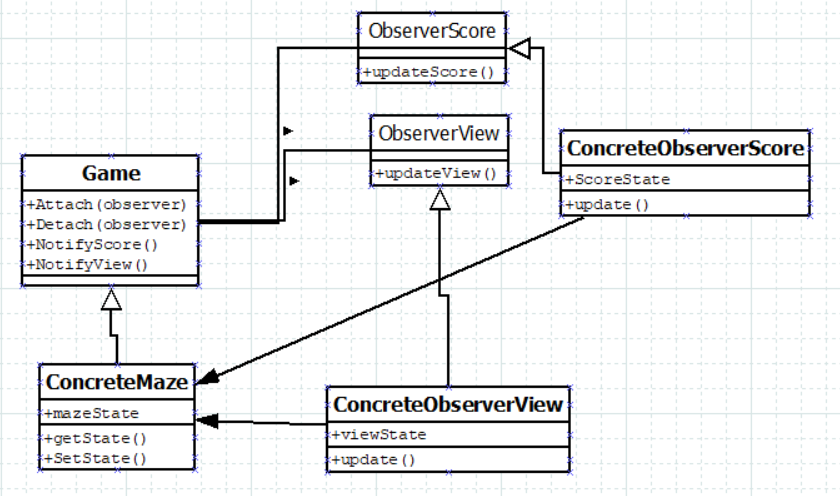
\includegraphics[scale=.5]{Observer.png}
\caption{How we will update the GUI}
\label{Game play}
\end{figure}
We chose the observer pattern because it allows us to customize the maze immediately on change.
\begin{figure}[ht!]
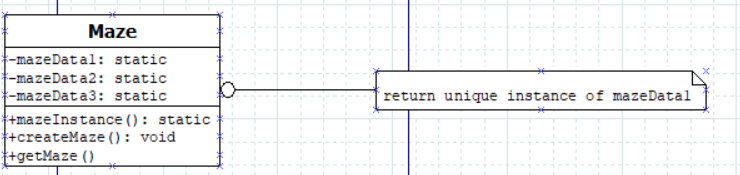
\includegraphics[scale=.5]{Singleton.png}
\caption{How we will handle the three instances of the maze}
\label{Maze instance}
\end{figure}
We chose the Singleton pattern to control the number of instances of the maze.
\clearpage
\subsection{Design Patterns Used}
\begin{enumerate}
\item Singleton
\item Observer
\end{enumerate}


\section{Results}
The result of our project is sad. We barely accomplished half of the work. We were unable to meet the minimum requirements. In summary, we have a half implemented maze game
This section will start out a little vague, but it should grow as your project evolves.  With each deliverable you hand in, give me a final summary of where your project stands.  By the end, this should be a reflective section discussing how many of your original goals you managed to attain/how many desired use cases you implemented/how many extra features you added.

\subsection{Future Work}
Future work, we will delete all copies of the game, and forget this catastrophe ever existed. In addition, this partnership will never happen again.




\begin{thebibliography}{1}

\bibitem{IEEEhowto:kopka}
H.~Kopka and P.~W. Daly, \emph{A Guide to \LaTeX}, 3rd~ed.\hskip 1em plus
  0.5em minus 0.4em\relax Harlow, England: Addison-Wesley, 1999.
\bibitem{Pullen}
Walter Pullen. \emph{Think Labyrinth},(2012).
\end{thebibliography}



\begin{IEEEbiography}{Michael Shell}
Biography text here.
\end{IEEEbiography}

% if you will not have a photo at all:
\begin{IEEEbiographynophoto}{John Doe}
Biography text here.
\end{IEEEbiographynophoto}

% insert where needed to balance the two columns on the last page with
% biographies
%\newpage

\begin{IEEEbiographynophoto}{Jane Doe}
Biography text here.
\end{IEEEbiographynophoto}





% that's all folks
\end{document}
